% 編集の過程で形式変換はよく行われるので、この過程で保たれる必要がある
Audio format conversions are frequently applied to media files during movie authoring.
To assure embedded annotations to be available through a whole authoring process, it is important that watermarks are kept detectable after format conversions.
% 変換後に保存された透かしの割合を計測することで強度を測定した
We evaluated the durability against conversions by measuring the proportion of preserved detectable watermarks in videos after applying a variety of format conversions.
% 10個のdetactableなwatermarkを含むwavファイルを圧縮したものにデコードを試みた
In this evaluation, an uncompressed audio file with ten detectable watermarks was converted to a compressed format using an audio encoder program and then watermark detection was applied to the converted file.
% 形式
MP3, Ogg Vorbis and AC-3 (also known as {\it Dolby Digital}) were selected as the compression algorithms because of their high popularities.
% 品質
For each formats, compressions were applied in four bit rate settings between 128 kbps and 320 kbps to examine the needed compression quality for preserving watermarks in each formats.
% 5種類のファイルに関して実験した
We measured the correct detection rates for five different audio files and calculated the means for each formats and quality settings.

According to the result shown in Figure \ref{fig:eval_conv}, watermarks can be preserved almost completely after a format conversion with Ogg Vorbis or AC-3 format and modest quality setting (over 192 kbps).
It suggests that our method can be used in practical movie authoring process since obviously satisfying these format requirements is not difficult.
% 一方でMP3が使えない
On the other hand, MP3 seems not suited for preserving watermarks even in a high bit rate setting, due to the characteristics of the compression algorithm that tend to discard high frequency components.
This fact means that recording instrument limited to store audio data in MP3-compressed format, such as several kinds of IC recorders and inexpensive video cameras, can not be used for embedding watermarks of AnnoTone.

% 結果
\begin{figure}[htbp]
 \begin{center}
  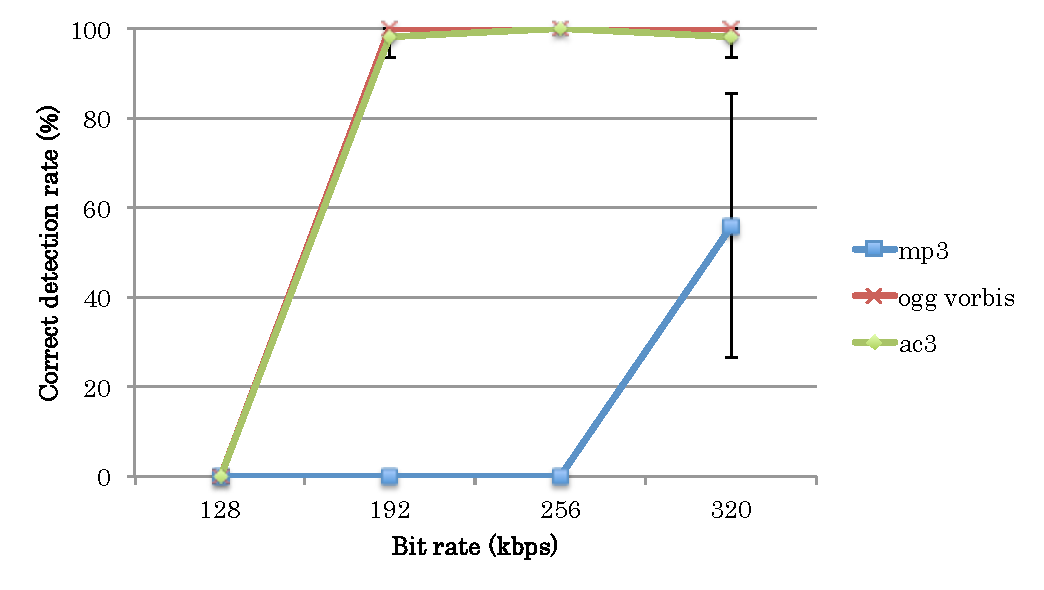
\includegraphics[width=120mm]{evaluation_conversion.pdf}
 \end{center}
 \caption{Average CDRs after format conversions for each compression settings.}
 \label{fig:eval_conv}
\end{figure}